\addtorecentlist{\textbackslash tableofcontents}

\begin{frame}[fragile]
    \frametitle{\lang,Contents,Inhoudsopgave,}
    
    \begin{columns}
        \begin{column}{0.5\textwidth}
            \begin{minted}[fontsize=\scriptsize,escapeinside=~~,highlightlines=6]{tex}
                ~~


                \begin{document}
                    \maketitle
                    \tableofcontents
        
                    \section{AA}
                    ...
                \end{document}
                ~~
            \end{minted}
        \end{column}
        \begin{column}{0.5\textwidth}
            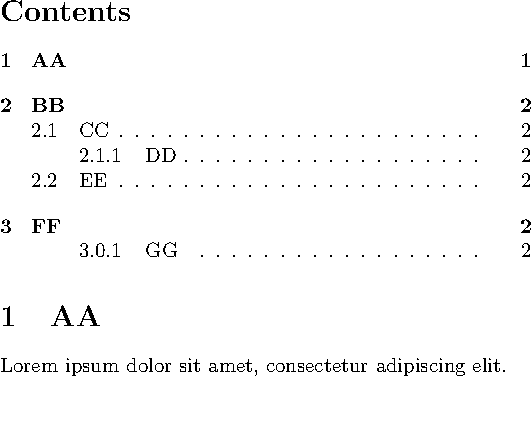
\includegraphics[width=\linewidth,height=0.8\textheight,keepaspectratio,page=1]{assets/tableofcontents.pdf}
            \vspace{-60pt}
        \end{column}
    \end{columns}
\end{frame}

\addtorecentlist{\textbackslash newpage}
\begin{frame}[fragile]
    \frametitle{\lang,Contents,Inhoudsopgave,}
    
    \begin{columns}
        \begin{column}{0.5\textwidth}
            \begin{minted}[fontsize=\scriptsize,escapeinside=~~,highlightlines=7]{tex}
                ~~

                
                \begin{document}
                    \maketitle
                    \tableofcontents
                    \newpage
                    
                    \section{AA}
                    ...
                \end{document}
            \end{minted}
        \end{column}
        \begin{column}{0.5\textwidth}
            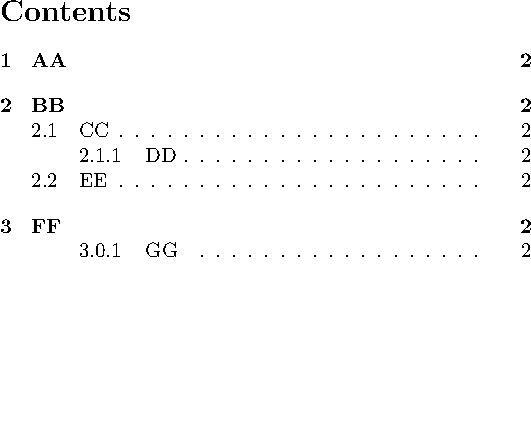
\includegraphics[width=\linewidth,height=0.8\textheight,keepaspectratio,page=1]{assets/tableofcontentswholepage.pdf}
            \vspace{-60pt}
        \end{column}
    \end{columns}
\end{frame}

\updatehighlight{
    name=accentB,
    remove={\newpage},
    add={babel,dutch},
    %
    name=default,
    add={\newpage}
}

\addtorecentlist{babel}

\begin{frame}[fragile]
    \frametitle{\lang,Contents,Inhoudsopgave,}
    
    \begin{columns}
        \begin{column}{0.5\textwidth}
            \begin{minted}[fontsize=\scriptsize,escapeinside=~~,highlightlines=1]{tex}
                \usepackage[dutch]{babel}
                ...
                
                \begin{document}
                    \maketitle
                    \tableofcontents
                    \newpage
                    
                    \section{AA}
                    ...
                \end{document}
            \end{minted}
        \end{column}
        \begin{column}{0.5\textwidth}
            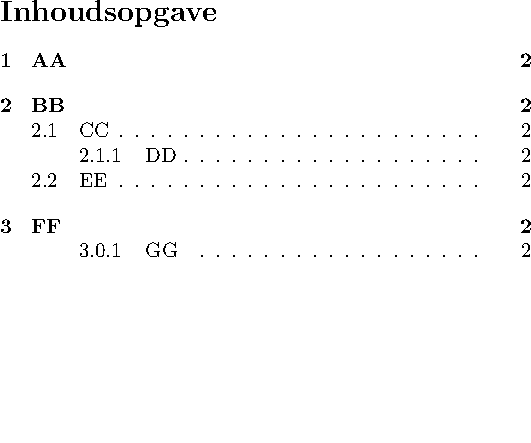
\includegraphics[width=\linewidth,height=0.8\textheight,keepaspectratio,page=1]{assets/tableofcontentsdutch.pdf}
            \vspace{-60pt}
        \end{column}
    \end{columns}
\end{frame}

\updatehighlight{
    name=accentB,
    remove={babel,dutch},
}
